\subsection{Casi d'uso}
In questa sezione sono riportati i casi d'uso relativi alla quarta versione dell'applicazione, sia in forma testuale che come diagramma UML.\bigskip 

In questa sezione sono riportati anche i casi d'uso che non sono soggetti a modifiche nella transizione dalla prima alla quarta versione dell'applicazione, al fine di presentarne una descrizione completa della struttura e del funzionamento.\bigskip

I casi d'uso specifici della quarta versione e non presenti nella terza sono:
\begin{itemize}
    \item Visualizzazione delle offerte chiuse
    \item Proposta di scambio
    \item Visualizzazione dell'ultimo messaggio
    \item Risposta di scambio
    \item Proposta di appuntamento
\end{itemize} \bigskip

Nella descrizione testuale di tutti i casi d'uso eccetto "Creazione configuratore", "Accesso configuratore", "Creazione fruitore" e "Accesso fruitore" è lasciato sottinteso il fatto che l'utente debba aver effettuato l'accesso al proprio profilo prima di poter proseguire con l'interazione descritta dal caso d'uso considerato: la scelta relativa all'azione da effettuare e di conseguenza del caso d'uso a cui far riferimento avviene infatti tramite un menu presentato all'utente solo dopo aver effettuato l'accesso, pertanto non sarebbe possibile richiedere di effettuare alcuna operazione che non sia la creazione di un nuovo profilo Configuratore o Fruitore o l'accesso a un profilo già esistente prima che venga presentato suddetto menu.\bigskip

Nella Tabella \ref{tab:Use Case 4.1} è riportato il caso d'uso testuale relativo all'accesso dell'utente configuratore al proprio profilo: l'utente interagisce con l'applicazione inserendo il proprio username e password; in questo caso d'uso, pertanto, è incluso il caso d'uso "Creazione configuratore" che viene invocato nella situazione in cui non esista ancora alcun utente o in cui un utente decida di non voler ritentare l'accesso a seguito dell'inserimento di credenziali errate ma piuttosto di creare un nuovo profilo.\bigskip

Nella Tabella \ref{tab:Use Case 4.2} è riportato il caso d'uso testuale relativo alla creazione di un nuovo profilo configuratore: l'utente riceve la comunicazione delle proprie credenziali temporanee, accede al proprio profilo e modifica le proprie credenziali a piacere (rispettando il vincolo relativo all'univocità dello username).\bigskip

Nella Tabella \ref{tab:Use Case 4.3} è riportato il caso d'uso testuale relativo alla creazione di una nuova gerarchia da parte dell'utente configuratore: l'utente, dopo aver effettuato l'accesso, interagisce con l'applicazione chiedendo di aggiungere nuove categorie oppure salvare la configurazione esistente; in questo caso d'uso, pertanto, sono inclusi i casi d'uso "Aggiunta categoria" e "Salvataggio dati", a cui si demandano i compiti relativi.\bigskip

Nella Tabella \ref{tab:Use Case 4.4} è riportato il caso d'uso testuale relativo alla visualizzazione di tutte le gerarchie presenti all'interno dell'applicazione da parte dell'utente configuratore; anche in questo caso d'uso è necessario che l'utente sia autorizzato ad accedere all'applicazione prima di poter interagire avanzando altre richieste.\bigskip

Nella Tabella \ref{tab:Use Case 4.5} è riportato il caso d'uso testuale relativo all'aggiunta di una categoria a una gerarchia; si tratta di un caso d'uso incluso in quello relativo alla creazione di una gerarchia.\bigskip

Nella Tabella \ref{tab:Use Case 4.6} è riportato il caso d'uso testuale relativo al salvataggio dei dati introdotti nell'applicazione dall'utente configuratore; anche in questo caso d'uso è necessario che l'utente sia autorizzato ad accedere all'applicazione prima di poter interagire avanzando altre richieste.\bigskip

Nella tabella \ref{tab:Use Case 4.7} è riportato il caso d'uso testuale relativo all'impostazione da parte dell'utente Configuratore dei parametri e delle informazioni di scambio. Le informazioni vengono salvate in modo permanente, in modo da consentirne la lettura ed eventuale modifica ad accessi successivi.\bigskip

Nella Tabella \ref{tab:Use Case 4.8} è riportato il caso d'uso testuale relativo alla creazione di un nuovo profilo fruitore: l'utente interagisce con l'applicazione inserendo il proprio username e password.\bigskip

Nella Tabella \ref{tab:Use Case 4.9} è riportato il caso d'uso testuale relativo all'accesso dell'utente fruitore al proprio profilo: l'utente interagisce con l'applicazione inserendo il proprio username e password, la cui correttezza viene verificata dall'applicazione.\bigskip

Nella Tabella \ref{tab:Use Case 4.10} è riportato il caso d'uso testuale relativo alla visualizzazione da parte di un utente fruitore delle informazioni di scambio e di nome e descrizione delle categorie radice delle gerarchie presenti nell'applicazione a seguito dell'inserimento da parte degli utenti configuratori.\bigskip

Nella Tabella \ref{tab:Use Case 4.11} è riportato il caso d'uso testuale relativo al ritiro di un'offerta da parte del fruitore: l'utente può scegliere un'offerta aperta e modificarne lo stato ritirandola.\bigskip

Nella Tabella \ref{tab:Use Case 4.12} è riportato il caso d'uso testuale relativo alla creazione di un'offerta da parte del fruitore: l'utente dovrà interagire con il sistema compilando i campi necessari per la corretta creazione della suddetta offerta.\bigskip

Nella Tabella \ref{tab:Use Case 4.13} è riportato il caso d'uso testuale relativo alla visualizzazione delle offerte relative ad una specifica categoria foglia da parte di un qualsiasi utente (sia fruitore che configuratore).\bigskip

Nella Tabella \ref{tab:Use Case 4.14} è riportato il caso d'uso testuale relativo alla visualizzazione da parte di un utente fruitore delle proprie offerte di baratto inserite, indipendentemente dal loro stato.\bigskip

Nella Tabella \ref{tab:Use Case 4.15} è riportato il caso d'uso testuale relativo alla visualizzazione da parte di un utente configuratore delle proprie offerte di baratto, il cui stato è \textit{Chiusa}, relative ad una categoria selezionata.\bigskip

Nella Tabella \ref{tab:Use Case 4.16} è riportato il caso d'uso testuale relativo alla creazione della vera e propria proposta di scambio da parte di un utente fruitore. L'utente seleziona la propria offerta aperta da accoppiare con un'altra offerta aperta nella stessa categoria, ma non di sua proprietà.\bigskip

Nella Tabella \ref{tab:Use Case 4.17} è riportato il caso d'uso testuale relativo alla visualizzazione dell'ultimo messaggio inviato dalla controparte coinvolta nello scambio. Il messaggio riguarda un'operazione di scambio prescelta dall'utente.\bigskip

Nella Tabella \ref{tab:Use Case 4.18} è riportato il caso d'uso testuale relativo alla risposta di scambio dell'utente che gestisce una proposta di scambio con un altro utente.\bigskip

Nella Tabella \ref{tab:Use Case 4.19} è riportato il caso d'uso testuale relativo alla proposta di appuntamento: l'utente in questo caso ha la possibilità di selezionare luogo, giorno e orario per fissare un appuntamento con la controparte coinvolta nello scambio.\bigskip 


In Figura \ref{fig:Use Case 4} è riportato il diagramma UML dei casi d'uso relativo alla quarta versione dell'applicazione. Dall'immagine possiamo ricavare facilmente che i casi d'uso \textit{sea-level}, ossia quelli corrispondenti agli obiettivi per cui l'utente interagisce con l'applicazione, sono:
\begin{itemize}
    \item Creazione di un nuovo profilo configuratore 
    \item Accesso a un profilo configuratore già esistente
    \item Creazione di una gerarchia di categorie
    \item Visualizzazione di tutte le gerarchie di categorie presenti nell'applicazione
    \item Salvataggio dei dati dell'applicazione
    \item Configurazione delle informazioni di scambio
    \item Visualizzazione delle offerte relative ad una specifica categoria
    \item Creazione di un nuovo profilo fruitore
    \item Accesso a un profilo fruitore già esistente
    \item Visualizzazione delle informazioni di scambio
    \item Visualizzazione delle offerte inserite personalmente dal fruitore
    \item Offerta di baratto
    \item Modifica dello stato dell'offerta  
    \item Visualizzazione delle offerte chiuse
    \item Proposta di scambio
    \item Visualizzazione dell'ultimo messaggio
    \item Risposta di scambio
\end{itemize}
Alcuni di questi casi d'uso \textit{sea-level} sono interpretabili come casi d'uso \textit{fish-level} laddove vengano inclusi da un altro caso d'uso al fine del raggiungimento dell'obiettivo per cui l'utente interagisce con l'applicazione.

Gli unici due casi d'uso che hanno natura esclusivamente \textit{fish-level} sono quelli relativi all'aggiunta di una nuova categoria a una gerarchia e della proposta di appuntamento per effettuare uno scambio, in quanto il primo dei due è incluso nel caso d'uso "Creazione gerarchia" mentre il secondo è incluso nel caso d'uso "Risposta scambio". Inoltre, i casi d'uso "Accesso configuratore", "Accesso fruitore" e "Salvataggio dati" sono inclusi in altri casi d'uso \textit{sea-level}, pertanto possono essere visti anche come casi d'uso \textit{fish-level} oltre che \textit{sea-level}.

\begin{figure}[ht]
\centering
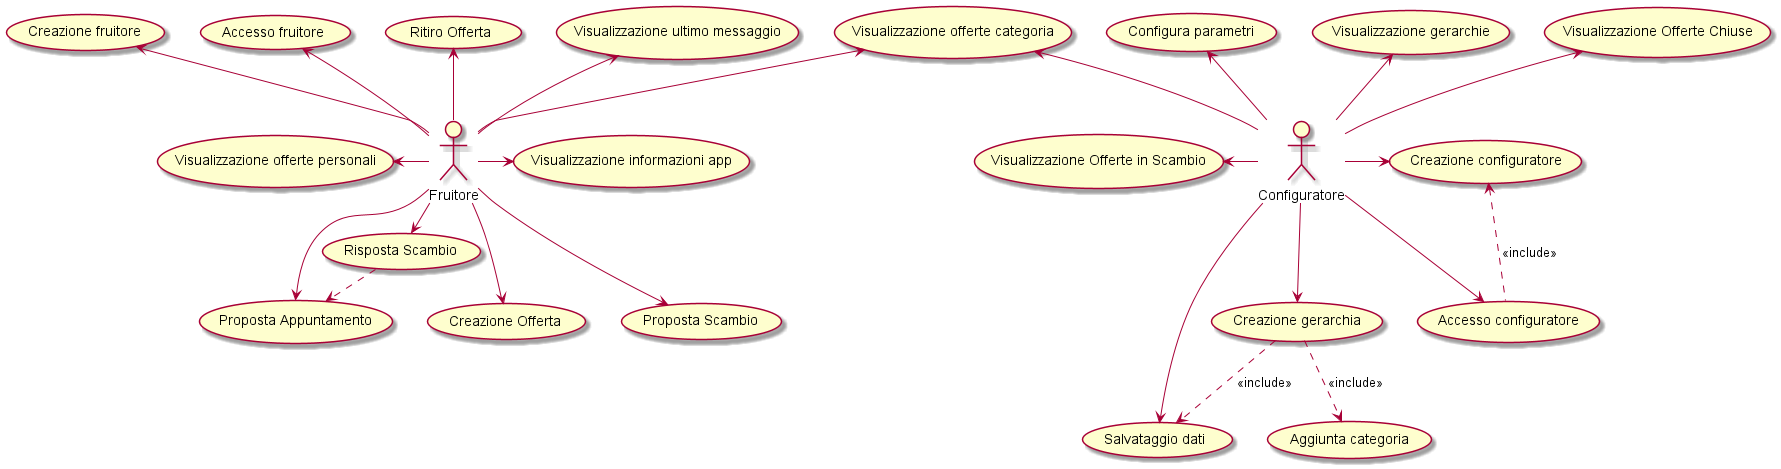
\includegraphics[width=17cm, height=5cm]{imagesV4/Use case diagram - Version 4.0.png}
\caption{\label{fig:Use Case 4}Diagramma UML dei casi d'uso - Versione 4}
\end{figure}\bigskip

